\section{Dimensional Reduction and Data Visualization}
\label{sec:dimRed}
In this section, we will begin our foray into unsupervised learning by way of data visualization. Data visualization methods are important for modelling as they can be used to identify correlated or redundant features along with irrelevant features (noise) from raw or processed data. For data involving a relatively small number of features, studying pair-wise correlations (i.e. pairwise scatter plots of all features) may suffice in performing a complete analysis. This rapidly becomes impractical for datasets involving a large number of measured features (such as images). \begin{mybox}{Dimensional Reduction}
	Thus, in practice, we often have to perform \emph{dimensional reduction}, namely, project or embed the data onto a lower dimensional space, which we refer to as the \emph{latent} space.\\
	A recurrent objective of dim. red. techniques is to preserve the relative pairwise distances (or defined similarities) between data points from the original space to the latent space.
\end{mybox}
Part of the complication of dim. red. lies in the fact that low-dimensional representations of high-dimensional data necessarily incurs information last.

\subsection{Some of the challenges of high-dimensional data}
\label{subsec:dimRedChallengesData}
\subsubsection{High-dimensional data lives near the edge of sample space}
Like one sees in statistical physics, for high-dimensional data, nearly only the surface of the $D$-dimensional sphere/cube/... describing it describes data points.

\subsubsection{Real-world data vs. uniform distribution}
Fortunately, real-world data is not random or uniformly distributed.\\
In facet, real data usually lives in a much lower dimensional space than the original space in which the features are being measured. This is sometimes referred to as the \emph{blessing of non-uniformity} (in opposition to the curse of dimensionality). 
\begin{example}
	For weakly interacting particles in stat. phys., one can describe them via thermodynamic variables and not via their microscopic degrees of freedom in phase space, this is the same idea.
\end{example}

\subsubsection{Intrinsic dimensionality and the crowding problem}
\begin{mybox}{Intrinsic dimensionality of the data}
	Qualitatively, this refers to the minimum number of dimensions (parameters) required to capture the signal in the data (to parametrize the data). 
\end{mybox}
\begin{mybox}{Crowding problem}
	Attempting to represent data in a space of dimensionality lower than its intrinsic dimensionality can lead to a \emph{crowding problem}. In short, because we are attempting to satisfy too many constraints (e.g. preserve all relative distances of the original space), this results in a trivial solution for the latent space where all mapped data points collapse to the centre of the map.
\end{mybox}
To alleviate this, one needs to weaken the constraints imposed on the visualization scheme. Powerful methods such as t-distributed stochastic embedding (t-SNE) and uniform manifold approximation and projection (UMAP) have been devised to circumvent this issue in various ways.


\subsection{Principal component analysis (PCA)}
\label{subsec:dimRedPCA}
\begin{mybox}{PCA}
A ubiquitous method for dimensional reduction, data visualization and analysis is \emph{Principal Component Analysis} (PCA). The goal of PCA is to perform an orthogonal transformation of the data in order to find high-variance directions. PCA is inspired by the observation that in many cases, the relevant information in a signal is contained in the directions with largest variance. This can be seen as ’fitting’ an ellipse to the data with the major axis corresponding to the first principal component (direction of largest variance).
\end{mybox}
Such PCA-based projections often capture a lot of the large scale structure of many datasets. Even without prior physical knowledge, one can extract relevant order parameters using a simple PCA-based projection.
\subsubsection{The theory}
\label{subsubsec:dimRedPCAtheory}
Consider $N$ data points, $\{\mx_1,\dots,\mx_N\}$ that live in a $p$-dimensional feature space $\mx_i \in \mR^p$. Denote the $N\times p$ design matrix as $\mX = [\mx_1,\dots,\mx_N]^T$ whose rows are the data points and columns correspond to different features, compare \ref{subsec:recipeML}. The $p\times p$ (symmetric) covariance matrix is therefore 
\be 
\label{eq:dimRedPCAcovMatrix}
\mathbf{\Sigma}(\mX) = \frac{1}{N-1} \mX^T \mX.
\ee 
notice that the $j$-th diagonal entry of $\mathbf{\Sigma}(\mX)$ corresponds to the variance of the $j$-th feature and $\mathbf{\Sigma}(\mX)_{ij}$ measures the covariance (i.e. connect correlation in the language of physics) between feature $i$ and feature $j$.\\
Via singular value decomposition (SVD), one finds
\be 
\mathbf{\Sigma}(\mX) = \mathbf{V} \left(\frac{\mathbf{S}^2}{N-1}\right) \mathbf{V}^T \equiv \mathbf{V}\mathbf{\Lambda} \mathbf{V}^T,
\ee 
where $\mathbf{V}$ contains (as its columns) the right singular vectors of $\mX$, and $\mathbf{\Lambda}$ is a diagonal matrix with eigenvalues $\lambda_i =s^2_i/(N-1)$ ($s_i$ are the singular values) in the decreasing order along the diagonal (i.e. eigendecomposition). It is clear that the right singular vectors of $\mX$ (i.e. the columns of $\mathbf{V}$) are principal directions of $\mathbf{\Sigma}(\mX)$, and the singular values of $\mx$ are related to the eigenvalues of the covariance matrix $\Sigma(\mX)$ via $\lambda_i$. To reduce the dimensionality of data from $p$ to $\tilde{p}<p$, we first construct the $p\times \tilde{p}$ projection matrix $\mathbf{V}_{\tilde{p}}$ by selecting the singular components with the $\tilde{p}$ largest singular values. The projection of the data from $p$ to $\tilde{p}$ is simply $\tilde{\mathbf{Y}}=\mX \mathbf{V}_{\tilde{p}}$. \\
The singular vector with the largest singular value (i.e. the largest variance) is referred to as the first principal component; the singular vector with the second largest singular value as the second principal component, and so on. An important quantity is the ration $\lambda_i/\sum_{i=1}^p \lambda_i$ which is referred as the \emph{percentage of the explained variance contained in a principal component}.\\
It is common in data visualization to present the data projected on the first few principal components. This is valid as long as a large part of the variance is explained in those components. Low values of explained variance may imply that the intrinsic dimensionality of the data is high or simply that it cannot be captured by a linear representation.

\subsection{Multidimensional scaling}
\label{subsec:dimRedMDS}
\begin{mybox}{MDS}
	Multidimensional scaling (MDS) is a non-linear dimensional reduction technique which preserves the pairwise distance or dissimilarity $d_{ij}$ between data points. There are two types of MDS. metric and non-metric.
\end{mybox}
\subsubsection{Metric MDS}
In metric MDS, the distance is computed under a pre-defined metric and the latent coordinates $\tilde{\mathbf{Y}}$ are obtained by minimizing the difference between the distance measured in the original space ($d_{ij}(\mx)$) and that in the latent space ($d_{ij}(\mathbf{Y})$):
\be 
\label{eq:dimRedMDS}
\tilde{\mathbf{Y}} = \arg \min_{\mathbf{Y}} \sum_{i<j} w_{ij} \abs{d_{ij} (\mX)-d_{ij}(\mathbf{Y})},
\ee 
where $w_{ij}\geq 0$ are weight values. The weight matrix $w_{ij}$ is a set of free parameters that specify the level of confidence (or precision) in the value of $d_{ij}(\mX)$. If Euclidean metric is used, MDS gives the same result as PCA and is usually referred to as classical scaling. Thus MDS is often considered as a generalization of PCA.

\subsubsection{Non-metric MDS}
In non-metric MDS, $d_{ij}$ can be any distance matrix. The objective function is then to preserve the ordination in the data, i.e. if $d_{12}(\mX) < d_{13}(\mX)$  in the original space, then in the latent space we should have $d_{12}(\mathbf{Y})< d_{13}(\mathbf{Y})$.

\subsubsection{General comment}
Both MDS and PCA can be implemented using standard Python packages such as Scikit. They are often among the first data visualization techniques one resorts to.

\subsection{t-SNE}
\label{subsec:dimRedTSNE}
It is often desirable to preserve local structures in high-dimensional datasets. However, when dealing with datasets having clusters delimitated by complicated surfaces or datasets with a large number of clusters, preserving local structures becomes difficult using linear techniques such as PCA\footnote{Non-linear techniques such as non-classical MDS, self-organizing map, Isomap and Locally Linear Embedding preserve local structures but fail to capture structures at the larger scale such as the clusters in which the data is organized.}.
\marginpar{Non-parametric hear means that it does not explicitly parametrize feature extraction required to compute the embedding coordinates. Thus it cannot be applied to find the coordinate of new data points.}
\begin{mybox}{t-SNE}
	Recently, $t$-stochastic neighbour embedding ($t$-SNE) has emerged as one of the go-to methods for visualizing high-dimensional data. $t$-SNE is a non-parametric method that constructs non-linear embeddings. Each high-dimensional training point is mapped to low-dimensional embedding coordinates, which are optimized in a way to preserve the local structure in the data.
\end{mybox}
\subsubsection{The theory}
The idea of stochastic neighbour embedding is to associate a probability distribution to the neighbourhood of each data (note $x\in \mR^p$, $p$ is the number of features):
\be 
p_{i|j} = \frac{\exp(-\norm{x_i-x_j}^2/2 \sigma^2_i)}{\sum_{k\neq i} \exp(-\norm{x_i-x_k}^2/2 sigma^2_i)},
\ee 
where $p_{i|j }$ can be interpreted as the likelihood that $x_j$ is $x_i$'s neighbour (thus we take $p_{i|i}=0$). $\sigma_i$ are free bandwidth parameters that are usually determined by fixing the local entropy $H(p_i)$ of each data point:
\be 
H(p_i) \equiv -\sum_j p_{j|i}\log_2 p_{j|i}.
\ee 
The local entropy is then set to equal a constant across \emph{all data points} $\Sigma = 2^{H(p_i)}$, where $\Sigma$ is called the \emph{perplexity}. The perplexity constraint determines $\sigma_i \forall i$ and implies that points in regions of high-density will have smaller $\sigma_i$.\\
\\
Using Gaussian likelihoods in $p_{i|j}$ implies that only points that are nearby $x_i$ contribute to its probability distribution. This ensures that the similarity, for nearby points is well represented but neglects the contributions of points far away. To alleviate this, we define a symmetrized distribution $p_{ij} \equiv (p_{i|j}+p_{j|i})/(2N)$. This \emph{guarantees} that $\sum_j p_{ij} >1/(2N)$ for all data points $x_i$, resulting in each data point $x_i$ making a significant contribution to the cost function to be defined below.
\begin{mybox}{tSNE}
	$t$-SNE constructs a \emph{similar} probability distribution $q_{ij}$ in a low dimensional latent space (with coordinates $Y=\{y_i\}, y_i \in \mR^{p^\prime}$, where $p^\prime <p$ is the dimension of the latent space):
	\be 
	\label{eq:dimRedTSNEprobdistr}
	q_{ij} = \frac{(1+\norm{y_i-y_j}^2)^{-1}}{\sum_{k\neq i} (1+\norm{y_i-y_k}^2)^{-1}}.
	\ee 
	The crucial point to note is that $q_{ij}$ is chosen to be a longtail distribution. This preserves short distance information (relative neighbourhoods) while strongly repelling two points that are far apart in the original space.\\
	In order to find the latent space coordinates $y_i$, $t$-SNE minimizes the Kullback-Leibler divergence between $q_{ij}$ and $p_{ij}$:
	\be 
	\label{eq:dimRedTSNECostfct}
	\mC(Y) = D_{KL} (p||q) \equiv \sum_{ij} p_{ij} \log\left(\frac{p_{ij}}{q_{ij}}\right).
	\ee 
	This minimization is done via GD (see \ref{sec:gd}).
\end{mybox}
Computing the gradient of \ref{eq:dimRedTSNECostfct}, we can see what the embedding cost-function $\mC$ is capturing
\begin{align}
	\label{eq:dimRedTSNEForce}
	\partial_{y_i} \mC&=\sum_{j\neq i} 4 p_{ij} q_{ij} Z_i(y_i-y_j) - \sum_{j\neq i} 4 q^2_{ij} Z_i(y_i-y_j)\nonumber \\
	&= F_{\text{attractive,}i} -F_{\text{repulsive,}i},
\end{align}
where $Z_i=1/(\sum_{k\neq i} (1+\norm{y_k-y_i}^2)^{-1})$. Notice that $F_{\text{attractive,}i}$ induces a significant attractive force only between points that are nearby point $i$ in the \emph{original space} since it involves the $p_{ij}$ term. Finding the embedding coordinates $y_i$ is thus equivalent to finding the equilibrium configuration of particles interacting through forces, compare \ref{eq:dimRedTSNEForce}.\\
\\
The $t$-SNE visualization cleanly separates all the clusters while certain clusters blend together in PCA for example. This is a direct consequence of the fact that $t$-SNE keeps nearby points close together while repelling points that are far apart, compare \ref{eq:dimRedTSNEForce}.

\subsubsection{Important properties of $t$-SNE}
\begin{enumerate}
\item $t$-SNE can rotate data:\\
The KL divergence is invariant under rotations in the latent space, i.e. $t$-SNE plots that are rotations of each other should be considered equivalent.
\item $t$-SNE results are stochastic.\\
In applying GD, the solution of different $t$-SNE runs depends on the initial seed and results in different outcomes.
\item \emph{$t$-SNE generally preserves short distance information}.\\
As a rule of thumb, one should expect that nearby points on the $t$-SNE map are also closeby in the original space, i.e. $t$-SNE tends to preserve ordination (but not actual distances).
\item \emph{Scales are deformed in $t$-SNE}.\\
Since a scale-free distribution is used in the latent space, one should not put too much emphasis on the meaning of the size of any clusters observed in the latent space.
\item \emph{$t$-SNE is computationally intensive}:\\
$\mO(N^2)$.
\end{enumerate}





\section{Clustering}
\label{sec:cluster}
This section is also concerned with unsupervised learning methods.\\
Unsupervised learning is concerned with discovering structure in unlabelled data (for instance learning local structures for data visualization \ref{sec:dimRed}). The lack of labels make unsupervised learning much more difficult and subtle than its supervised counterpart. What is somewhat surprising is that even without labels it is still possible to uncover and exploit the hidden structure in the data. Perhaps, the simplest example of unsupervised learning is clustering.
\begin{mybox}{Clustering}
 The aim of clustering is to group unlabelled data into clusters according to some similarity or distance measure. Informally, a cluster is though of as a set of points sharing some pattern or structure.\\
 Clustering finds many applications throughout data mining, data compression and signal processing. Clustering can be used to identify coarse features or high level structures in an unlabelled dataset.
\end{mybox}
The field of clustering is vast and there exists a flurry of clustering methods suited for different purposes. Some common considerations one has to take into account when choosing a particular method is the distribution of the clusters (overlapping/noisy clusters vs. well-separated clusters), the geometry of the data (flat vs. non-flat), the cluster size distribution (multiple sizes vs. uniform sizes), the dimensionality of the data (low vs. high dimensional) and the computational efficiency of the desired method (small vs. large dataset).


\subsection{Practical clustering methods}
\label{subsec:clusterPractical}
Throughout this section we focus on the Euclidean distance as a similarity measure.

\subsubsection{$K$-means}
\label{subsubsec:clusterPracticalKmeans}

Consider a set of $N$ \emph{unlabelled} observations $\{\mx_n\}^N_{n=1}$ where $\mx_n\in \mR^p$ and where $p$ is the number of features. Also consider a set of $K$ cluster centres called the cluster \emph{means}: $\{\mathbf{μ}_k\}^K_{k=1}$, with $\mathbf{μ}_k\in \mR^p$, which we'll compute ’empirically’ in the clustering procedure. The cluster means can be though of as the representatives of each cluster, to which data points are assigned. 
\begin{mybox}{$K$-means set-up}
	$K$-means clustering can be formulated as follows: given a fixed integer $K$, find the cluster means $\{\mathbf{μ}\}$ and the data point assignments in order to minimize the following objective function
	\be
	\label{eq:clusterPracticalKmeansCostfct}
	\mC(\{x,\mathbf{μ}\}) = \sum_{k=1}^K \sum_{n=1}^N r_{nk} ( \mx_n - \mathbf{μ}_k)^2,
	\ee
	where $r_{nk} \in \{0,1\}$ is a binary variable called the \emph{assignment}. The assignment $r_{nk}$ is $1$ if $x_n$ is assigned to cluster $k$ and $0$ otherwise. Notice that $\sum_k r_{nk}=1 \forall n$ and $\sum_n r_{nk}\equiv N_k$, where $N_k$ is the number of points assigned to cluster $k$. The minimization of this objective function can be understood as trying to find the best cluster means such that the variance within each cluster is minimized.
\end{mybox}
In physical terms, $\mC$ is equivalent to the sum of the moments of inertia of every cluster. The cluster means $\mathbf{μ}_k$ correspond to the centres of mass of their respective cluster.
\begin{mybox}{$K$-means algorithm}
	The $K$-means algorithm alternates between two steps:
	\begin{enumerate}
		\item \emph{Expectation}: Given a set of assignments $\{r_{nk}\}$, minimize $\mC$ w.r.t. $\mathbf{μ}_k$. Taking a simple derivative and setting it to zero yields the following update rule:
		\be 
		\mathbf{μ}_k = \frac{1}{N_k} \sum_n r_{nk} \mx_n.
		\ee 
		\item \emph{Maximization}: Given a set of cluster means $\{\mathbf{μ}_k\}$, find the assignments $\{r_{nk} \}$ which minimizes $\mC$. Clearly, this is achieved by assigning each data point to their nearest cluster-mean:
		\be
		r_{nk} = \left\{ \begin{array}{ll}
		1 & \text{if } k=\arg \min_{k^\prime} (\mx_n-\mathbf{μ}_{k^\prime})^2 \\
		0& \text{otherwise}.
		\end{array}\right\}
		\ee 
	\end{enumerate}
Practically, the algorithm should terminate when the change in the objective function from one iteration to another becomes smaller than a pre-specified threshold.
\end{mybox}
A nice property of the $K$-means algorithm is that it is guaranteed to converge.\footnote{To see this, one can verify explicitly (by taking second-order derivatives) that the expectation and assignment step respectively always decrease $\mC$. Thus, since $\mC$ is bounded from below, the two-step iteration of $K$-means \emph{always} converges to a local maximum of $\mC$. Since $\mC$ is generally a non-convex function, in practice one usually needs to run the algorithm with different initial random cluster centre initializations and post-select the best local minimum.} The complexity is $\mO(KN)$ per iteration and is thus scalable to very large datasets.\\
A common drawback of $K$-means is the following:\\
If the true clusters have very different variances (spreads), $K$-means can lead to spurious results since the underlying assumption is that the latent model has uniform variances.

\subsubsection{Hierarchical clustering: Agglomerative methods}
\label{subsubsec:ClusterPracticalHierarchical}
Agglomerative clustering is a bottom up approach that starts from small initial clusters which are then progressively merged to form larger clusters.
\begin{figure}[h!]
	\centering
	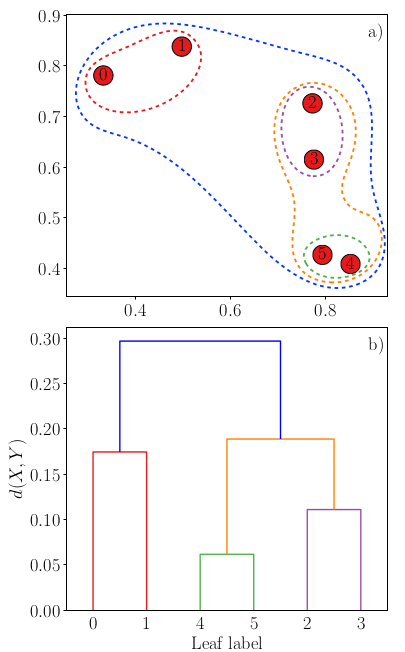
\includegraphics[width=0.4\linewidth]{gfx/HierarchicalCLustering}
	\caption{}
	\label{fig:hierarchicalclustering}
\end{figure}





















